\subsection{Карты Карно}
Дана функция (ДНФ):
$$
F=(A\overline{B} + \overline{A}B)
$$

Необходимо сделать: 
\begin{itemize}
\item Таблицу истинности:
\item СДНФ: Для написания формулы по таблице истинности необходимо выписать конъюнкции 
аргументов тех наборов, на которых функция равна 1, причем аргумент, равный 0, входит 
в конъюнкцию с отрицанием, а аргумент, равный 1 -- без отрицания. Затем следует соединить 
все образованные конъюнкции знаком дизъюнкции.
\item СКНФ: При составлении формулы {\it по 0} записываем дизъюнкции аргументов тех 
наборов, где $f=0$. Аргумент в дизъюнкцию входит с отрицанием, если в наборе он равен 1. 
Все составленные дизъюнкции объединяем операцией конъюнкции.
\item Карты Карно: Прямоугольник делится на равные части столько раз, сколько переменных. 
Деление осуществляется вертикальными или горизонтальными линиями. Одна половина функции 
лежит в области, где аргумент равен 0, другая -- где аргумент равен 1. Над областью (или 
слева от области) где аргумент равен 1, проводится черта и подписывается имя аргумента. 
Каждый квадрат карты соответствует набору таблицы.
\end{itemize}

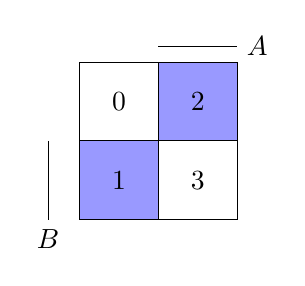
\begin{tikzpicture}
\draw (0,0) rectangle (1,1) rectangle (2,0)
(0,1) rectangle (1,2) rectangle (2,1)
(1,2.2) -- (2,2.2) node[right] {$A$}
(-0.4,1) -- (-0.4,0) node[below] {$B$};
%\fill[red!90!white,thick] (0,0) rectangle (1,1);
\filldraw[blue!40!white, draw=black] (0,0) rectangle (1,1) (1,1) rectangle (2,2);
\draw (0.5,1.5) node {0} (1.5,1.5) node {2}
(0.5,0.5) node {1} (1.5,0.5) node {3};
\end{tikzpicture}

\begin{table}[ht]
  \centering%центрируем таблицу	
\begin{tabular}{@{} cccccc @{}}
\toprule
\multirow{2}{*}{в 10-тичной системе}&\multicolumn{2}{|c|}{аргументы}& 
\multicolumn{2}{|c|}{в алгебраической форме}\\
\cmidrule{2-5}&
\multicolumn{1}{|c|}{A}&\multicolumn{1}{|c|}{B}& \multicolumn{1}{|c|}{дизъюнкции}&
\multicolumn{1}{|c|}{конъюнкции}\\
\midrule 
0 & 0 & 0 &  $A+B$ & $\bar{A}\bar{B}$ \\
1 & 0 & 0 &  $A+\overline{B}$ & $\overline{A}B$\\
2 & 1 & 0 &  $\overline{A}+B$ & $A\overline{B}$\\
3 & 1 & 1 & $\overline{A}$+$\overline{B}$ & $AB$ \\ 
\bottomrule
\end{tabular}
\caption{Элементарные конъюнкции и дизъюнкции}\label{tab:table_init}
\end{table} 

